\documentclass[12pt]{article}
%Gummi|065|=)
\usepackage{amsmath, amsfonts, amssymb}
\usepackage[margin=0.5in]{geometry}
\usepackage{xcolor}
\usepackage{graphicx}

\usepackage{pifont}
\usepackage{amsmath}

\newcommand{\off}[1]{}
\DeclareMathSizes{20}{30}{20}{18}

\newcommand{\two }{\sqrt[3]{2}}
\newcommand{\four}{\sqrt[3]{4}}
\newcommand{\red}{\begin{tikz}[scale=0.25]
\draw[fill=red, color=red] (0,0)--(1,0)--(1,1)--(0,1)--cycle;\end{tikz}}
\newcommand{\blue}{\begin{tikz}[scale=0.25]
\draw[fill=blue, color=blue] (0,0)--(1,0)--(1,1)--(0,1)--cycle;\end{tikz}}
\newcommand{\green}{\begin{tikz}[scale=0.25]
\draw[fill=green, color=green] (0,0)--(1,0)--(1,1)--(0,1)--cycle;\end{tikz}}

\newcommand{\sq}[3]{\draw[#3] (#1,#2)--(#1+1,#2)--(#1+1,#2+1)--(#1,#2+1)--cycle;}

\usepackage{tikz}

\newcommand{\susy}{{\bf Q}}
\newcommand{\RV}{{\text{R}_\text{V}}}

\title{Scratchwork: Divergences}
\author{John D Mangual}
\date{}
\begin{document}

\fontfamily{qag}\selectfont \fontsize{12.5}{15}\selectfont

\maketitle

\noindent It's time to get serious.  I can nearly put it together myself.  \\ \\
How do I review this proof without it degenerating into some kind of recitation fo facts? One of my critiques of analytic number theory is that\dots it doesn't look like number theory.  If I spend all this effort to prove the Prime Number Theory\dots I already believed it was true! \\ \\
I started to look for arguments where the connection to prime factorization or to Geometry or Probablity or any other branch of Math.\footnote{If I express someone of my aggravation, and provide a partial demonstration / answer, that could be new.}  Talking to professors, I'm pretty much out of luck. They are satisfied with the current arguments.  They are professionals, I'm not.\\ \\
Try to imagine if Hollywood or a Hip-Hop label adopted the garbled narrative style of a Math Textbook.  To me, Mathematics has been a giant bait-and-switch.  They sold me one result, I got completely another.   \\ \\ 
I'm trying not to do that to you.  \\ \\
Zagier proves PNT as a series of facts.  He introduces 3 functions:
\begin{itemize}
\item $\displaystyle \zeta(s) = \sum_{n=1}^\infty \frac{1}{n^s}$
\item $\displaystyle \Phi(s) = \sum_{p > 1} \frac{\log p}{p^s}$
\item $\displaystyle \theta(s) = \sum_{p < x} \log p $
\end{itemize}
If you a sequence of numbers $a_n$ here are three different numbers you could assign to that sequence:
$$ \{ a_n\}_{n=1}^\infty \mapsto \sum_{n=1}^\infty a_n 
\text{ or } 
\{ a_n\}_{n=1}^\infty \mapsto \sum_{p > 1} a_p 
\text{ or }
\{ a_n\}_{n=1}^\infty \mapsto \sum_{p < x} a_p $$
One is a sum over \textit{all integers} another is a sum over \textit{all primes} and the other is over \textit{primes less than $x$}.  This is what Hardy saw: all these are just ways of assigning numerical averages to sequences of numbers.  Some are better behaved than others. \\ \\
He starts to prove a sequence of facts.

\newpage

\noindent \textbf{\#1} The Euler Product: this sum over integers $n$ is also sum over primes $p$. 
$$ \zeta(s) = \sum_{n=1}^\infty \frac{1}{n^s} = \prod_p \frac{1}{1 - p^{-s}}$$
This falls out of Unique Factorization, which calls out of the Euclidean Algorithm.  Lurking in the background is the statment $\mathrm{Spec}(\mathbb{Z}) = \{ \text{primes}\}$, in the event we choose to use scheme. \\ \\
\textbf{\#2} If we subtract the pole at $s = 1$, this function extends holomorphically to $\mathrm{Re}(s) > 0$.  
$$ \zeta(s) - \frac{1}{s-1} $$
This statement is loaded.  I never noticed it before.  There is already ``analytic continuation": 
$$ \zeta \big( \frac{1}{2} \big) = \sum_{n=1}^\infty \frac{1}{\sqrt{n}} = 
1 + \frac{1}{\sqrt{2}} +  \frac{1}{\sqrt{3}} +   \frac{1}{\sqrt{4}} + \dots =\infty $$
We'll say, rather bluntly, that it equals infinity.  Leaving more refined information later. \\ The numbers never get small enough. And we only subtract off a small amount:
$$ \zeta(\frac{1}{2}) - \frac{1}{\frac{1}{2}-1} = \infty + 2 $$
and perhaps this is why I dislike analytic number theory.  We have to competely change our way of adding - without any mention at all - just because of this one small thing.
$$  \zeta(s) - \frac{1}{s-1}
= \sum_{n=1}^\infty \frac{1}{n^s} -  \int_1^\infty  \frac{dx}{x^s} 
= \sum_{n=1}^\infty \int_n^{n+1} \left( \frac{1}{n^s} - \frac{1}{x^s} \right) \, dx < \infty $$
so for each term, we can subtract off the excess, and get a finite number. \\ \\
\textbf{\#3} $\theta(x) = O(x)$.  Could we be a little more obnoxious here?
$$   \sum_{p < x} \log p  = O(x)$$
if $f(x) = O(x)$ this means $f(x) \leq C x $ and we don't care about the constant.  Or how about this?
$$ \frac{1}{x} \sum_{p < x} \log p  = O(1) $$
which is saying this number is finite.\footnote{There are many theories to try to include ``infinite numbers" but none of them have been successful.  Even in the time I have left graduate school, there are peole trying and doing pretty well.  And others, trying to remove all the divergences.}  No surprises here.   \\ \\
\textbf{\#4} $\zeta(1 + it) \neq 0$ and we have holomorphic function on $\mathrm{Re}(s) \geq 1$.  
$$ \frac{\zeta'(s)}{\zeta(s)} = \sum_{n=1}^\infty \frac{\Lambda(n) }{n^s} =
\sum_{p> 1} \frac{\log p}{p^s - 1} = 
 \sum_{p > 1} \frac{ \log p }{p^s}  + (\text{ finite number })(s)$$
 
\newpage 

\noindent \textbf{\#5} $\to$ \textbf{\#6}
$$ \left[ \int_1^\infty \frac{\theta(x) - x}{x^2} \, dx < \infty \right] \to \left[ \theta(x) \sim x \right]  $$
This notation is aggravating for a number of reasons.  Usually I define the symbol $\theta$ to mean something else:
$$  \theta(q) \neq \sum_{n=1}^\infty q^{n^2}$$
and I still don't know the preicse meaning of $A\sim B$ (instead of  $A \asymp B$). Here it means $\frac{A}{B} \to 1$. \\ \\ 
If I phrase it differently setting $\frac{1}{x} \theta(x)   = f(x)$ and say:
$$ \left[ \int_1^\infty \frac{f(x)-1}{x} \, dx < \infty \right] \to \big[ f(x) \sim 1 \big]  $$
I don't know if this is precise but I am a lot happier. That leaves us to prove item \#5. \\ \\
One great question here is why it was possible to write down the integral of $\theta(x)$. Between the $\int$ sign and the word ``holomorphc" a lot of things have gotten swept under the rug.  However, correctly. \\ \\
\textbf{\#5} Tauberian theorems all have statements like ``obviously that thing should converge" and then it does converge.  And we could try to imagine functions where the implication does not hold. \\ \\
In Chapter 1 of Titchmarsh, Tauber's Theorem was stated like this:
$$ \Big[ \lim_{x \to 1} \sum_{n = 0}^\infty a_n \, x^n = s \Big] \stackrel{a_n = o(n^{-1})}{\to\,\to \, \to} \Big[ \sum_{n = 0}^\infty a_n = s \Big] $$
and it as the converse to \textbf{Abel's Theorem} which is why these are called Abelian and Tauberian theorems.
$$ \Big[ \sum_{n = 0}^\infty a_n = s \Big]  \to 
\Big[ \lim_{x \to 1} \sum_{n = 0}^\infty a_n \, x^n = s \; (\text{uniformly}) \Big]  $$
and we would confront an unknown series and we would apply one of these litmus tests and if we were careful it yielded a positive result.  \\ \\
$$ \left[ g(z) = \int_0^\infty f(t) e^{-zt} \, dt \text{ \textbf{holomorphic} on }\mathrm{Re}(z) \geq 0\right] \to \left[ g(0) = \int_0^\infty f(t) \, dt \right] $$
More belaboring the obvious.  This is why we like Complex Analysis.  At least in principles, theorem yield under $\mathbb{C}$ that wouldn't under $\mathbb{R}$. And this is our replacement for pages and pages of Tauberian theorems.  \\ \\
It remains to prove item \#5, philosophize about the Cauchy-Riemann equations, meditate about many proofs whose statements are modeled after the Prime Number Theorem.  This could be done later. \\ \\
What could be done now, is to figure out why Sauzin talks about Zagier-Newman's paper in 2014 in this discussion on {\color{red!50!green!50!orange}\textbf{resurgence}} and {\color{blue!80!white}\textbf{1}}-{\color{blue!80!white}\textbf{summability}}.  This is me taking something at face-value, when I shouldn't. \\ \\
Zagier had taken Newman's short proof and made it even shorter:
$$ \left[ (\mathcal{L}\phi )(z) = \int_0^\infty e^{-z t }\phi(t) \, dt \text{ holo. }\mathrm{Re}(z) \geq 0 \right]\to \left[  \int_0^T \phi(t) \, dt = (\mathcal{L}\phi)(0)\right]  $$
I guess it's time to say something about {\color{green!50!orange}holomorphic extension}. The number $(\mathcal{L}\phi)(0)$ was not defined by writing an integral as it was for $(\mathcal{L}\phi)(z)$ with $\mathrm{Re}(z) > 0$.  Here's one definition:\footnote{The contour $C$ should contain the origin $0$.}
$$ g(0) = \frac{1}{2\pi i } \oint_C f(z) \, e^{zT} \, \left( 1 + \frac{z^2}{R^2} \right) \, \frac{dz}{z}  $$
and this integral is the same, regardless of the value of $T \in \mathbb{R}$.  We could even set $T = 0$ and leave it out.  On the other hand, 
$$ g_T(0) = \int_0^T f(t) \, dt = \oint_C f(z) \, e^{zT} \, \left( 1 + \frac{z^2}{R^2} \right) \, \frac{dz}{z} $$
and now the statement looks really tautological, because we wish to show
$$ \lim_{T \to \infty} \big| g(0) - g_T(0) \big|  = 0 $$
for some \textbf{bounded} and \textbf{locally integrable} function.  These are big words, whose number-theory content I don't fully understand.  Yet
$$ f(t) = \theta(e^t) - e^t \hspace{0.125in}\text{ and }\hspace{0.125in}
g(z) = \frac{1}{z}\sum_{p > 1} \frac{\log p}{p^s}  - \frac{1}{z-1}$$
Hopefully I wrote the Laplace transform identities correctly:
\begin{itemize}
\item $\displaystyle \mathcal{L}(t \,\phi) = \frac{d\phi }{dz}$
\item $\displaystyle (e^{ct} \,\mathcal{L}\phi)  = \phi(z + c)$ 
\item $\displaystyle \mathcal{L}(1 * \phi) = z^{-1}\phi(z) $ 
\item $\displaystyle \mathcal{L}\left( \frac{d\phi}{dt} \right) = z \phi(z) - \phi(0) $ 
\end{itemize}
There's nothing ``divergent" about this discussion, but I have to think about it some more. \\ \\
For one thing I'd be concerned about writing an Laplace trasnform integral
$$ \dots $$
$C$ is a semicircle contour $|z| = R$ and $\mathrm{Re}(z) > -\delta$, moved ``infinitesially" over the real l ine.

\newpage

\noindent The Gamma function: 
$$ \Gamma(z+1) t^{-(z+1)} = \int_0^\infty x^z e^{-xt} \, dx $$
is the Laplace transform of a power function.  Therefore if we write down an operator like:
$$ g(0) = \frac{1}{2\pi i } \oint_{C} f(z) \, e^{zT} \, \left( 1 + \frac{z^2}{R^2} \right) \, \frac{dz}{z} $$
we might ask for the inverse Laplace transform of $g$ and hopefully it will be something like $f$.
$$ \sum_{n=0}^\infty a_n z^n \stackrel{\mathcal{L}^{-1}}{\to} \sum_{n=0}^\infty a_n \frac{x^n}{n!}$$ 
The problem is unequivocally solved, but there are still maybe some interesting problems about how all the different part work.  I am still reading.  There's a Stirling series:
$$ \log \big[ \Gamma(z)  \big]
\sim \sqrt{2\pi z} (z/e)^z  
\sum \frac{B_{2k}}{2k(2k-1)} z^{-2k+1}  $$
and this is this is also the resurgent expansion of $\log n!$ This is looking like the start of a  very different discussion than the one by Newman+Zagier.

\begin{thebibliography}{}

\item Terence Tao 
\\ \textbf{The Euler-Maclaurin formula, Bernoulli numbers, the zeta function, and real-variable analytic continuation} 
\texttt{http://bit.ly/2cyNB3H}
\item GH Hardy \textbf{Divergent Series}  Oxford University Press, 1949/1973.
\item EC Titchmarsh \textbf{Theory of Functions} \texttt{https://archive.org/details/TheTheoryOfFunctions}
\item Simon Rubinstein-Salzedo \textbf{Could Euler have conjectured the prime number theorem?} \texttt{ arXiv:1701.04718}
\item Andrew Granville, Adam J Harper, K. Soundararajan \textbf{A more intuitive proof of a sharp version of Hal\'{a}sz's theorem} \texttt{arXiv:1706.03755}

\item Serge Lang \textbf{Algebraic Number Theory} \\
(Graduate Texts in Mathematics \#110) Springer, 1970.

\item J\"{u}rgen Neukirch. \textbf{Algebraic Number Theory} \\ (Grundlehren der mathematischen Wissenschaften \#322) Springer, 1999.

\item David Sauzin \textbf{Introduction to 1-summability and resurgence} \texttt{arXiv:1405.0356}

\item Don Zagier \textbf{On Newman's Short Proof of the Prime Number Theorem} \texttt{http://people.mpim-bonn.mpg.de/zagier/files/doi/10.2307/2975232/fulltext.pdf}

\end{thebibliography}

\newpage

\noindent \textbf{7/10}  To keep things interesting, it's time to include more examples of problems that can be solved with technique.  I doubt anyone really understands it the first time around but the algebraic number theory textbooks lift statements about $\mathbb{Q}$ and $\mathbb{Z}$ and $\zeta(s)$ to 
\begin{itemize}
\item all number fields
\item arithmetic progressions
\item Grossencharakters ( I don't know what they are but it sounds really big ! )
\end{itemize}
Any ``lift" that behaves this nicely is called a \textbf{functor}.  We can write $L$-functions for very deep objects such as varieties and schemes and motives, cuspital automorphic representations, etc.  Finally these things can be read in terms of \textbf{category theory}.\footnote{My understanding is category theory can be taught to pre-schoolers.  It's the type of reasoning we do before there is any concept of symbol or number.  We just look at objects and connections between them.  We manipulate them with our hands.  In a Mathematician's mind these are the basic object.  In practice, there's still a lot of work to be done.  Mostly it looks like nonsense.} \\ \\
All of their solutions will have the same spirit: they will solve the problem but either something terrifying was swept under the rug - in a relatively safe correct way, mind you - or the proof was write in such advanced language it is no longer possible to corroborate if their argument is correct. One is left with more questions than answers. \\ \\
Part of why contributing to math seems to be difficult is the criterion of ``novelty".\footnote{What if we were looking for tall things?  5-foot-6 is hardly considered tall, it is the typical height.  If someone is 6 foot, they are pretty tall.  Even in a small town, the tallest person might be over 6-foot-6.  The tallest people in the world well over 7 feet and suffer from genetic disorders.  These things are also to subject to verification and to dispute.  Perhaps being first is not the best thing? Or very meaningful? Sultan Kosen (Turkey) and I share the same birthdya of 10 December.} After much digging and probing, the exercise I had proposed, to show the equidistribution of prime numbers in $\mathbb{Z}[i]$ is very carefully and beautifully done in Edmund Hlawka's textbook. \\ \\
This doesn't prelude me finding yet another technique that solves this style of problem.  There's a field called \textbf{Additive Combinatorics} that I am really enjoying.  However, which theorem do I use?  They don't really deal with Prime Number Theorem -- in their group, they will use an example called {\color{red!50!green!50!blue}Szemeredi Theorem} about arithmetic progressions in sequences of numbers.  Prime numbers very sparse compared to arithmetic progressions (or any sequence of numbers that occurs with some ``regularity").  If I'm not mistaken we'd strengthen Szemeredi's Theorem and start to strip away all the extraneous numbers until we get arithemtic sequences of primes. \\ \\
And that's just one idea.    When we are ready we are free to write our own. There are many other fish in the sea. \\ \\
These theorems seem to be about the same strength:
\begin{itemize}
\item Hardy Littlewood Tauberian Theorem
\item Weierstrass Approximation Theorem
\item Hairy Ball Theorem (from Topology)
\item Gambler's Ruin
\end{itemize}
and the Prime Number Theorm will evade all of these. So I tried to have a glimpse of 

\newpage

\noindent I've begun to speculate these other theorems are of the same strength:
\begin{itemize}
\item Wiener-Ikehara Tauberian Theorem
\item Euler-Maclaurin Summation Formula
\item The Heat Kernel
\end{itemize}
I currently do not have the technical resources or follow-through to solve it.  Until then we have Newman + Zagier. \\ \\ \\ \\ \\
\textbf{7/10} Time to get off the soapbox. Let's widen the panorama a bit with Edmund Hlawka's discussion bit.  He did exactly what I was going to do: he read Newman's proof and solved it for $K = \mathbb{Z}[i]$.  Perhaps I can try $\mathbb{Z}[\sqrt{-5}]$ which has a non-trivial class number $h = 2$.
$$ 6 = 2 \times 3 = (1 - \sqrt{5}) \times (1 + \sqrt{-5}) $$ 
Or $\mathbb{Z}[i]$. Maybe let's try to write down an $L$-function that counts 
$$ \sum_{n \geq 0} \frac{ \# \Big\{ (a,b): a^2 + b^2 = n \text{ and } 0 < \tan^{-1}( \frac{b}{a}) < \frac{\pi}{3} \Big\} }{ n^s } $$
This blog is full of errors.  I doubt even if I wrote this one correctly.  Off we go\dots \\ \\
Neukich is a great and reliable textbook to introduce algebraic number theory. He only shows there are infinitely many primes in arithmetic sequences (which he does for all number fields).   He covers other things! Serge Lang, writes in rather austere manner, yet he obtains for us.  Now, if I find the guy's writing a bit spare, perhaps there's a Lemma I can contribute that creates a more vivid set of images. \\ \\
I hypothesize there are two kinds of singularies that are connected by the Prime Number Theorem.  The zeta function has a \textbf{pole} at $s = 1$, as $\zeta(1) =  \sum \frac{1}{n} = 1 + \frac{1}{2} + \frac{1}{3} + \dots = \infty $
$$ \Bigg[ \Gamma(z+1) \sim \sqrt{2\pi z} \, (z/e)^z \, (\dots) \Bigg] \leftrightarrow \Bigg[ \zeta(s) = \frac{1}{s-1} + \dots  \Bigg] $$
For simplicity $\Gamma(n+1)=n!$ is called the \textbf{factorial}.  The function $(z/e)^z$ has \textbf{essential singularities} both at $z = 0$ (where it behaves like $0^0$) and $z = \infty$ (where it behaves like $\infty^\infty$).  Even our friend, the exponential function has some sly behavior near $z = \infty$:
$$ e^{\frac{1}{z}} \to e^\infty \text{ near }z=0 $$
Sauzin in his discussion of 1-summability and resurgence proceeds quite casually.  Yet, every time we invoke the Stirling formula, a singularity quite worse than this exists in between the lines.
$$ e^{z \, \log z  } = e^{ (re^{i\theta}) \, \log (re^{i\theta}) } 
= e^{ (re^{i\theta}) \, \big( \log r + i\theta + 2\pi i k \big) }  $$
Hopefully I am still on topic here if I say there's no good way to assign a phase angle if $r \to \infty$

\newpage

\noindent That might explain why the real analsis techniques are so difficult. The essential singularity for $(\infty)!$ seem much more difficult than the pole for $\zeta(1)$.  Holomorphic functions - if we can obtain them - simplify life tremendously. These seemingly endless benefits, I wonder how long could last. \\ \\
To be fair $(\infty + \epsilon  \, e^{i\theta})!$ where $\epsilon \ll 1$ is very tiny.  And $\zeta(1 + \epsilon  \, e^{i\theta} ) = \frac{1}{0} +  {\color{blue}\mathbf{1}}\times i \theta \,\epsilon $.  Neither of these describe any information at all a priori.  You know, off the bat.  Maybe it's a separate thing to show in either case 
that $\frac{1}{x} \sum_{n < x} \Lambda(n) = {\color{blue}\mathbf{1}}$. A pole is much easier than an essencial singularity. \\ \\
Sauzin doesn't explicitly say, his discussion of resurgence and 1-summability kind of mixes the two. \\ \\
\textbf{7/11} Algebraic number theorists write in this rather baroque way, here's a statement:
\begin{itemize}
\item There are infinitely many primes in arithmetic progressions $\{ an+b : n \in \mathbb{Z}\}$.  
\end{itemize}
This could be true if $(a,b) = 1$ were \textbf{relatively prime}. So there are infinitely many primes in the sequence:
$$ 1, 4 = 2 \times 2, 7, 10 = 5 \times 2, 13, 16 = 2^4, 19, 22 = 2 \times 11, \dots  $$
As an data analyst -- as a person living in the Bronx where, to be honest -- nobody gives a damn\footnote{They wear t-shirts saying ``No f*cks given."}, {\color{orange!80!green}why do primes matter}?  When I did a K-means clustering or linear regression, did prime factorization play a role? I found just a little bit on Wikipedia\footnote{\texttt{https://en.wikipedia.org/wiki/Almost\_{}periodic\_{}function}}
\begin{quotation}
 A theorem of Kronecker from diophantine approximation can be used to show that any particular configuration that occurs once, will recur to within any specified accuracy: if we wait long enough we can observe the planets all return to within a second of arc to the positions they once were in.
\end{quotation} 
In other words, any dynamical system - any collection of observations over time - even if we don't understand it very well, or have any equations to model we can find observations at two different times that are early identical. \\ \\
A common strategy for finding two near-identical states is the \textbf{pigeonhole principle} it can be played very primitively (let me find two things that are kind of the same) or it can be done more finessed.  It always takes imagination expand a limited set of observations into enough data for the pigeonhole principle.  Or there might be too much data for it to be meaningful. \\ \\
We could talk about \textbf{Poincare Recurrence}
\begin{quotation}
Let $(X, \mathcal{X}, \mu, T) $ be a measure preserving system and let $E\in \mathcal{X} $ be a set of positive measure. Then 
$$ \limsup_{n \to \infty} \; \mu \big( E \cap T^n E\big) \geq \mu(E)^2 $$
in particular the set of $n$ with $E \cap T^nE$ non-empty 
$$ \# \big\{  n : E \cap T^n E \neq \varnothing \big\}  = \infty $$
\end{quotation}
so if we watch the a part system evolve, it will coincide withitself infintely many times.  And it will always do so.  And these kind of results can be played in increasingly refined manners.  Or existing results can be viewed as refined pigeonhole principles. 

\newpage

\noindent \textbf{7/12} I said the prime number theorm is now part of a paradigm.  Heré s a few more statements of this kind:
\begin{itemize}
\item There are infinitely many primes in arithmetic sequences $ak+b$ with $(a,b)=1$ relatively prime
\item the primes are equidistributed among residue classes.  There are as many $4k+1$ primes as $4k+3$ primes.
\item the primes in $\mathbb{Z}[i]$ point in evenly distributed directions as $p \to \infty$.  This is true for any number field $K$.
\item Sato-Tate conjecture (we could connect the simplest cases to the Gaussian primes, i.e. primes in $\mathbb{Z}[i]$).
\item Chebotarev Density Theorem
\item the primes in any number field have a density
\item the number $(a,b,c)$ such that $n = a^2 + b^2 + c^2$ point in evenly spread directions in the sphere.  This is relatively knew and quite difficult, but it can be turned into statements about $L$-functions at $z = 1$ or $z = \frac{1}{2}$. 
\end{itemize} 
There are modular forms for days, and if we work them out carefully there should be many elementary statements such as these. 
After that we I don't know of any statements where the modular forms, L-functions and elementary appraches clearly coincide.  \\ \\
I'm not being too original.  If I start with Fermat's Theorem 
$$ p = a^2 + b^2 \leftrightarrow p = 4k+1 $$
there are many novel proofs such the one by Zagier or Heath-Brown, I can try to find equidstiribution results from there. \\ \\
Famous 3-manifold toologist, Ian Agol answered my question on Math Stackexchange once.\footnote{\texttt{https://math.stackexchange.com/questions/225175/structure-of-x2-xy-y2-z2-integer-quadratic-form}} I asked how to look for the generators of an integer Lie group
$$ O\big( x^2 + xy + y^2 - z^2 , \mathbb{Z} \big) \stackrel{?}{\subseteq} GL(3, \mathbb{Z}) $$
My friend Seth Blumberg wrote his senior thesis on it.  Perhaps I'm looking too much into a novelty, but I thought he did a great job! \\ \\
Anyway the statement of the Chebotarev density is written in a complicated way, but here's data on the factorization of a polynomial $X^4 - X^2 - 1$ and $X^4 - X - 1$ over each prime.\footnote{\texttt{http://websites.math.leidenuniv.nl/algebra/Lenstra-Chebotarev.pdf}}
$$ \begin{array}{l|ccccc}
 & (4) & (1, 3) & (2,2) & (1,1,2) & (1,1,1,1 ) \\ \hline \\
X^4 - X^2 - 1 & \frac{1}{4} & 0 & \frac{3}{8} & \frac{1}{4} & \frac{1}{8} \\\\
X^4 - X \,\;- 1 & \frac{1}{4} &\frac{1}{3} & \frac{1}{8} & \frac{1}{4} & \frac{1}{24}
\end{array} $$
Soon I'll leave the topic of prime numbers, until I decide how they connect to general data.

\newpage

\noindent \textbf{7/15} I found this textbook that promises both geometry and analysis in their discussion of the Prime Number Theorem and they will even extend up to Gaussian primes.  Fermat's theorem says a prime $p = 4k+1 \in \mathbb{Z}$ can be written as the sum of two squares $p = a^2 + b^2$.  This can also be read as saying that primes $p = 4k+1$ that live in $\mathbb{Z}$ ``split" when they move up to $\mathbb{Z}[i]$ since we can write: $p = a^2 + b^2 = (a+bi)(a-bi)$. \\ \\ \includegraphics[width=2in]{pnt-resurgence-01.png}  \\
He says the chronology is this way:
\begin{itemize}
\item Chebyshev tries to prove the theorem in {\color{orange!50!green}1850}.
\item Mertens offers some estimates in {\color{orange!50!green} 1870}.
\item Riemann, Hadamard and De la Valee Poussin offer complex analysis proof in {\color{orange!50!green}1896}.
\item Norbert Wiener proves PNT in {\color{orange!50!green}1932} with difficult theory of distributions.
\item Selberg and Erdos offer ``elementary" proofs resorting to enormous trickery,  {\color{orange!50!green} 1947}.
\item Newman offers simplified Tauberian theorem leading to proof in {\color{orange!50!green} 1980}.
\end{itemize}
and then we really are done.  There are a few other proofs missing from this list using \textbf{sieve theory} but also now we have automorphic forms and the Langlands program.  However, those more advanced statements are written entirly using L-functions and representation theory and there's nobody to turn them into basic number theory. \\ \\
Hard to believe, Hlawka's discussion will be a only a few pages (some of which we've already done; we're doing it over).  I needed to come up with a ``rubric" of how far I need to go to prove statements of this type.  In my opinion, it got way, way out of hand.   \\ \\
It turns out there very good reasons for it.  And there \textit{is} room for new discussion.   \\ \\
So, we can do Hlawka. Hua Loo Keng will give an excellent (economical !!) discussion of the full Tauberian itself and he even exhibits a few of the culprits for us!

\vfill


\begin{thebibliography}{}

\item Simon Rubinstein-Salzedo \textbf{Could Euler have conjectured the prime number theorem?} \texttt{ arXiv:1701.04718}
\item Andrew Granville, Adam J Harper, K. Soundararajan \textbf{A more intuitive proof of a sharp version of Hal\'{a}sz's theorem} \texttt{arXiv:1706.03755}

\item Serge Lang \textbf{Algebraic Number Theory} \\
(Graduate Texts in Mathematics \#110) Springer, 1970.

\item J\"{u}rgen Neukirch. \textbf{Algebraic Number Theory} \\ (Grundlehren der mathematischen Wissenschaften \#322) Springer, 1999.

\item David Sauzin \textbf{Introduction to 1-summability and resurgence} \texttt{arXiv:1405.0356}

\item Edmund Hlawka \textbf{Geometric and Analytic Number Theory} (Universitext) Springer, 1991.

\end{thebibliography}

\newpage

\noindent \textbf{7/23} The 3-squares bound can be stated without reference to modular forms.  By Weyl's criterion, equidistribution just requires that the averages over the sphere tend to zero.  \\ If $u \in L^2 ( \text{Sphere})$:
$$  \frac{1}{r_3(n)} \sum_{(a,b,c) \in V_3(n)} u \big( a, b, c \big) \ll n^{-1/28} $$
That number $r_3(n) = \# \{ (a,b,c) : n = a^2 + b^2 + c^2 \}$ has a lot of variance. Sometimes it can be written with other symbols. \\ \\
The modular forms theory is telling us these averages are related to each other in a non-trivial way.\footnote{Every time we use the word non-trivial, there's a meditation on the notion of \textbf{zero} of nothingness.} Here is exhibit A. \\
\includegraphics[width=4.5in]{pnt-resurgence-02.png} \\ \\
If I feel it doesn't say anything, I have to articulate what is missing.  If I improve on his result, I have to say what I improved.  Obviously it's a big mess, but I don't know what it says, I don't know how to make it better and I don't know how to explain what I improved about it. Our task could be to ameliorate it gradually, perhaps to almost nothing.   A basic, concrete goal is to improve on the exponent of $- \frac{1}{28}$. I've read many smart competent pros wince at improving this exponent. They state it as a given, it starts to sound like bluffing.  \\
\includegraphics[width=4.5in]{3-squares.png} \\
Do these numbers look equidistributed?  It actually looks like there's quite a bit of patterns.  And that could be our way out. \\ \\
For starters of all the stles of proof I listed in the previous, this looks more like the Erdos-Selberg styles of proof than anything.  Completely elementary and completely chaotic.  Perhaps it has an analogue that will yield some type of ``improvement". \\ \\
And of course, there are newer ideas not on the previous list.

\newpage 

\noindent \textbf{Edmund Hlawka}  \\ \\
towards Equidistribution of primes in $\mathbb{Z}[i]$. \\ \\


\newpage 

\noindent \textbf{Henryk Iwaniec} \\ \\
Devious Kloosterman sums. \\ \\
First of all.  Why Kloosterman?  Here is Iwaniec's theorem: 
\begin{quotation} 
Let $a_n$ be the $n$-th Fourier coefficient of a cusp form $f(z)$ of weight $k = \frac{1}{2} + \ell \geq \frac{5}{2}$ for the group $\Gamma = \Gamma_0(N)$ with $N \equiv 0 \pmod 4$, normalized by 
$$ \langle f, f \rangle = \int_{\Gamma \backslash \mathbb{H}} \big| f(z) \big|^2 \; y^k \; \frac{dx \, dy}{y^2 } = 1$$ 
Then for $n$ square-free, we have (the implied constant for $\ll$ depends only on $k$)
$$  a_n \ll n^{k/2 - 2/7} \tau (n) \big( \log 2n \big)^2 $$
\end{quotation}
When I was a kid, a teacher threw me a physics book and it say that symmetries ``determine" constraints on an object.  The example they gave was a box.  And if you rotate the box $90^\circ$ in any direction it looks the same.   So it must be a cube. \\ \\
Iwaniec does not tell us how to obtain such objects in any way.  Yet, if we do find an equation:
$$ f(z) = \sum_{n=1}^\infty a_n \, e \big( n z \big) 
= \sum_{n=1}^\infty a_n \, q^n $$
The numbers $a_n$ are constrained quite-a-bit, once we understand the jargon:
\begin{itemize}
\item ``cusp form" means $a_0 = 0$
\item modular form means $f(z) y^{k/2}$ is invariant under the symmetries of $\Gamma$
\item $\Gamma$ is a ``congruence subgroup" such as $\big\langle z \mapsto z + 1, z \mapsto - \frac{1}{4z} \big\rangle$
\item $n$ is square-free, e.g. $n \neq 18 = 2 \times 3^2 $ but $n = 35 = 5 \times 7$ is OK.
\end{itemize}
This is enough to put a strict relationship on all of the $n$, but where do we find such a thing? \\ Duke borrows his from Goro Shimura. \\ \\ If $u \in L^2 (\text{Sphere})$ is a \textbf{spherical harmonic} of degree $\ell$:
$$ \theta(z; u) = \sum_{m \in \mathbb{Z}^3} u(m) \; e \big(z \,|(a,b,c)|^2 \big)  =  \sum_{m \neq  0} m^{\ell/2} \; r_3(m) \; \left[ \frac{1}{r_3(m)} \sum_{ \{(a,b,c): a^2 + b^2 + c^2 = m  \}} u\left(\frac{a}{m},\frac{b}{m},\frac{c}{m} \right) \right] e \big( |m| z \big)  $$
is a modular form of weight $ k = \ell + \frac{3}{2}$ on $\Gamma_0(4) \subseteq \mathrm{SL}(2, \mathbb{Z})$. Shimura says the proof is easy. \\ \\
It's a surprise to me we didn't lose modularity in the process of adding all these bells and whistles.  It was found by trial-and-error, these days we know it's part of the \textbf{theta correspondence}.  \\ \\
We can sort of, by decree, illustrate or prove these things are modular forms of whatever congruence group.  Someone with less knowledge (like me) could try running through all the formulas and try to write down formulas involving the $a_n$ that express the symmetry. \\ \\
It's not obvious that $\theta(z; u)$ is a modular form.  And only vague hints.  We know that Mumford's ``Lectures on Theta" contains some generalized theta functions, but he doesn't go quite as far as Goro Shimura. \\ \\
Q: \\ 
{\color{orange!50!green}{Do coeffients of modular forms obtained by theta functions, count solutions to an equation}}? \\ \\
We are so far up the ladder of abstraction, perhaps the word ``counting" would become something else as well?  Also, we are up for some intensive french reading on the paper of Waldspurger, who will turn all these modular forms into L-functions. It overwhelms my ability to scoop from Spanish cognates. \\ \\
The L-function version is connected to these low-fat estimates of Burgess:
$$ L(\frac{1}{2} + it, \chi_D ) \ll |D|^{3/16 + \epsilon} $$
that's getting ahead of ourselves. \\ \\
Henryk Iwaniec proved his theorem in 1987.  The final steps are difficult.  The earlier steps are - as of 2002 in his textbook - \textbf{Spectral Methods of Automorphic Forms} which summarize his lectures at \textit{Universidad Aut\'{o}noma de Madrid}.  He very suggestively opens his notes with the Gauss circle problem:
\begin{quotation} If $k \in C_0^\infty(\mathbb{R})$ is a smooth and \_\_\_\_ function:
$$ \sum_{\ell=1}^\infty r(\ell) \; k(\ell) = \sum_{\ell=1}^\infty r(\ell) \; \widehat{k}(\ell)$$
where $r(\ell)$ counts the lattice points on a circle.  
$$ r(\ell) = \# \Big\{ (m,n): m^2 + n^2 = \ell  \Big\}  $$
We could also count the lattice points ``near" a circle.  That's a huge deal too.
$$ \widehat{k} (\ell) = \pi \int_0^{+\infty} k(t) \, J_0 \big( 2pi \sqrt{\ell \, t} \big) \, dt$$
This is called the {\color{red!50!orange}{Hankel transform}}.
\end{quotation}
These lattice points count eigenvalues of the operator $D = \frac{\partial^2 }{\partial x^2} + \frac{\partial^2 }{\partial y^2} $ (this is on flat space $\mathbb{R}^2$), and we obtain the Weyl law.  $\# \{ x : \lambda (x ) \leq T \}  = T/4\pi + O(T^{1/3}) $
\vfill
So the weirdness has already come in.  Doing very natural things, we have both the apple and the orange.  Then it gets somewhat political.  Doing all these explorations some parts of it were ``new" but I couldn't tell you which part. 

\newpage \noindent
Henryk will provide 4 or 5 chapters of discussion in his book.  I feel his discussion is missing connections to Combinatorics.  And there I will be!
\begin{itemize}
\item the Weyl averages get encoded as theta functions (separated by their \textbf{degree})
\item cusp forms at each degree form a finite dimensional vector space ( an expansion exists, but we don't really know more info) 
\item a spanning set (not really a basis) can be written in terms of Poincar\'{e} series. 
$$ P_m(z; k, \Gamma) =  \sum_{\tau  \in \Gamma_\infty \backslash \Gamma }
j(\tau, z)^{-2k} e(m\tau z)  $$
\item Through clumsy and rather involved manipulations of Kloosterman sums we will obtain our bound.
\end{itemize}
Items \#1 thru \# 3 are in a textbook and have excellent disussion.  In my opinion, he left all the good parts out.  \\ \\
{\color{red!50!orange!50!green} \textbf{Wikipedia}} \\ \\
A superficial internet search shows that Poincar\'{e} series generalize both Eisenstein series and Theta functions.  \\ \\
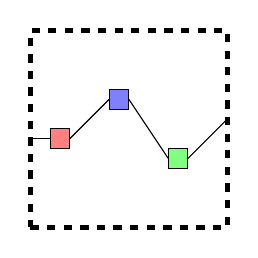
\begin{tikzpicture}[scale=0.25]

\draw[dashed, line width = 2] (0,0)--(10,0)--(10,10)--(0,10)--cycle;

\draw[fill=red!50!white] (1,4)--(2,4)--(2,5)--(1,5)--cycle;

\draw[fill=blue!50!white] (4,7)--(5,7)--(5,6)--(4,6)--cycle;

\draw[fill=green!50!white] (7,3)--(8,3)--(8,4)--(7,4)--cycle;

\draw (0,4.5)--(1,4.5);

\draw (2,4.5)--(4,6.5);

\draw (5,6.5)--(7,3.5);

\draw (8,3.5)--(10,5.5);

\end{tikzpicture} \\ \\
I have no idea what Poincare series are and when I look them up - even in fairly advanced textbooks - they are nowhere to be found.
\begin{itemize}
\item Tom Apostol \textbf{Modular Functions and Dirichlet Series in Number Theory} GTM \#41 (1990) 
\item Tom Apostol \textbf{Introduction to Analytic Number Theory} UTM, (1976)
\end{itemize} 
The books were published 14 years apart, so we can see how slow the progress is.  And neither of the textbooks discuss Poincar\'{e} seres.  \\\\
Iwaniec's paper was written in 1987 and his book - covering aspects of his work - was published in 2002, for a 15 years gap. \\ \\
Progress is slow.  These objects look elementary and - with a stroke of insight - can be done in a basic way, but it takes so long to figure out.  \\ \\
What is a Poincar\'{e} series?  And why does it appear now in relation to Eisenstein series, theta series, cusp forms and other modular objects? \\ \\
One problem: {\color{orange!50!black!50!green} we have alredy exhausted all the explicit construction of modular forms in this short paragraph}.  In my opinion, I don't know how this field proceeds without anything to go on.

\newpage

\noindent Henryk sketches tell me that we \textbf{don't} know a lot about Poincare series.  Modular forms are rare to begin with, but we reason about them as if they were everywhere.    \\ \\
\textbf{1} A modular form $f(z)$ is called a {\color{blue}cusp form} if it vanishes on each cusp of $\Gamma$. The cusp of $\mathbb{H}/\Gamma$ are the parts that touch the real axis, $\mathbb{R} + 0i \subseteq \mathbb{C}$.  The space of cusp forms $S_k(\Gamma)$ is a \textbf{finite dimensional} Hilbert space  with inner product:
$$\langle f,g \rangle = \int_{\Gamma \backslash \mathbb{H}}  f(z) \, \overline{g(z)} \, y^k \, \frac{dx \, dy}{y^2} \hspace{0.25in}\text{ with }\hspace{0.25in}\frac{dx \, dy}{y^2}=dA $$
It's rare to find examples of these cusp forms and even rarer to find explicit computations.  I'd have to tell you what I mean by ``special value" in a way that's consistent with our common sense. \\ \\
The space of cusp forms is spanned by Poincare series.  These are indexed by $m \in \mathbb{Z}$
$$ P_m (z; k , \Gamma ) = \int_{\Gamma \backslash \mathbb{H}} j (\tau, z)^{-2k} \, e(m \tau z) $$
Basically this is the \textbf{method of images} we are reflecting an ordinary function over the boundaries of three circular mirrors and hoping for the best.  In fact, these series will be divergent! \\ \\
Poisson summation was also proven using Method of images.  There was function $f(x): \mathbb{R} \to \mathbb{C}$ and then we considered the sum of infinitely many shifted copies of itself:
$$  \sum_{n \in \mathbb{Z}} f(x) \stackrel{?}{<} \infty  $$
and we hoped the series didn't accumulate too much or have derivatives that are too big.  Then we could take the Fourier series of itself:
$$  \sum_{n \in \mathbb{Z}} f(x)  = \sum_{n \in \mathbb{Z}} \widehat{f}(-n) \, e^{2\pi i \, n x} $$
and there is confusion if we mean $\widehat{f}(n)$ as a Fourier transform of  $f: \mathbb{R} \to \mathbb{C}$ or of the sum $g(x) = \sum_{n \in \mathbb{Z}} f(x+n): \mathbb{R}/\mathbb{Z} \to \mathbb{C}$. I would argue this enriched Poisson summation over $\Gamma \backslash \mathbb{H}$ has not been explored very carefully. \\ \\
Iwaniec's original construction was likely derived from the theta function:
$$  \theta(z) = \sum_{n \in \mathbb{Z}} q^{n^2} \hspace{0.25in}\text{with}\hspace{0.25in} q = e^{2\pi i \, n z}$$
and his modular forms are built from ``theta multipliers" and all of this groups are congruence groups $\Gamma = \Gamma_0(N)$ with $N \equiv 0 \pmod 4$.  Obviously, $\theta(z+1) = \theta(z)$, so perhaps we need:
$$ \theta(z + \frac{1}{4}) = \sum_{n \in \mathbb{Z}} q^{n^2}
= \sum_{n \in \mathbb{Z}} e^{2\pi i n^2 \, (z + \frac{1}{4})} 
= \sum_{n \in \mathbb{Z}} q^{n^2}
e^{\frac{1}{2}\pi i n^2 } $$
the number $e^{\frac{1}{2}\pi i n^2 } = \pm 1$.  Quitely, the exercise of designing these modular forms has turned into one of twisting actions of $SL(2, \mathbb{Z})$ on various function spaces. 

\newpage

\noindent Like a child, where do moudular forms come from? Far as I can tell, we'll never get an answer.  And I'm a little bit shocked that Iwaniec only does $\Gamma = \Gamma_0(4M)$.  I'm a total beginner and I can think of other Fuchsian groups, even non-congruence groups.  \\ \\ 
Let's fix one of Iwaniec's typos:
$$ j(\tau, z) = \theta(\tau z) / \theta(z) \hspace{0.125in}\text{instead of}\hspace{0.125in}
\Theta(\tau z) / \theta(z) $$
which could also be common notation for something (e.g. Siegel modular form, or a vector-valued theta function).  And the formula for $j(\tau, z)$ comes from hard work.  It's really built from (three) formulas:
\begin{eqnarray*}
\sum_{n \in \mathbb{Z}} e(n^2 (z+1) ) &=& \sum_{n \in \mathbb{Z}} e(n^2 z ) \\ \\
\sum_{n \in \mathbb{Z}} e(n^2 \frac{1}{4z+1} ) &=& 1 \times \frac{1}{\sqrt{4z+1}} \times \sum_{n \in \mathbb{Z}} e(n^2 z ) \\ \\
\sum_{n \in \mathbb{Z}} e(n^2 \frac{1}{4z-1} ) &=& i \times \frac{1}{\sqrt{4z-1}} \times \sum_{n \in \mathbb{Z}} e(n^2 z )
\end{eqnarray*}
Poisson Summation can also be made to look like modular invariance with $z \mapsto - \frac{1}{4z} $ \,:
$$ \sum_{n \in \mathbb{Z}} e(n^2 \times - \frac{1}{4z} ) = 1 \times \frac{1}{2\sqrt{z}} \times \sum_{n \in \mathbb{Z}} e(n^2 z ) $$ 
This is worse than Physics class.  Everyone (rather competently) charging through the equations.  I was like Stop! Stop! Look! Reason!! Think!! \\ \\
All this ``unpacking" that I've been doing, does not improve the Iwaniec bound in any way but at least we understand better. \\ \\
Our group is defined by:
$$ \Gamma_0(N) = \left\{  \left( \begin{array}{cc} a & b \\ c & d \end{array}\right) 
: c \equiv 0 \pmod N\right\} $$
and a holomorphic function $f(z)$ is a modular form of weight $k$ when
$$ f( \gamma z) = j(\gamma, z)^{2k}f(z)$$
with $z \in \mathbb{H} $ and $\gamma \in \Gamma_0(N)$. \\ \\
The theta function $\theta(z)$ is a  modular form of weight $k = \frac{1}{2}$ and $\Gamma = \Gamma_0(4)$. \\ \\
Eisenstein series are the $m = 0$ case of Poincar\'{e} series.  Here we need all of them $m \in \mathbb{Z}$:
$$ P_m(z; k , \Gamma) =   \sum_{\gamma \in \Gamma_0 \backslash \Gamma } \frac{\# \times e(m \tau z)}{|cz+d|^k} \hspace{0.125in} = \Bigg|_{m=0} \hspace{0.125in} E(z; k ,\Gamma)  \sum_{\gamma \in \Gamma_0 \backslash \Gamma }  \frac{\#}{|cz+d|^k} $$
the cusps are indexed by $\Gamma_0 \backslash \Gamma$ basically they are $\{ (c,d) : \mathrm{gcd}(c,d) = 1 \}$ pairs of relatively prime numbers, sitting on the real axis $\mathbb{R}$ at the edge of the hyperbolic space $\mathbb{H}$.

\newpage \noindent It remains to write down the Fourier coefficient of the Poincare series for all $m \in \mathbb{Z}$:
$$ P_m( z; k , \Gamma) = \sum_{\tau \in \Gamma_0 \backslash \Gamma } j(\tau, z)^{-2k} \, e^{m\tau z} $$
\textbf{Q}: How to write our enriched theta functions in terms of these Poincare series?  At least we know an expansion exists:
$$ \theta(z; u) = \sum_{m \geq 0} \left[ \frac{1}{V_3(m)} \sum_{x \in V_3(m)} u(x)  \right]  e(mz) $$
We know the answer involves Bessel functions:
$$ \widehat{P}_m (n; k , \Gamma) = \left( \frac{n}{m} \right)^{\frac{k-1}{2}} 
\left\{  \delta_{mn} + 2\pi i^{-k} \sum_{c \equiv 0 \pmod N}^\infty \frac{1}{c}
J_{k-1} \left( \frac{4\pi \sqrt{mn}}{c}\right) K(m,n; c) \right\} $$
the Kloosterman functions themselves have been generalized.  At this point, it's better ot consult Iwaniec's book from 2002 for something closer to the state of the art.  For now:
$$ K(m,n;c) = \sum_{d \pmod c} \varepsilon_d^{-2k} \left( \frac{c}{d} \right) e \left(  \frac{m \overline{d} +  n d}{c} \right) $$
Since this is the Analysis blog, I can say there are two factors:
\begin{itemize}
\item $J_k$ about the average behavior of cubic lattices in $\mathbb{Z}^3$
\item $K(m,n;c)$ about the number theoretic-behvior of these lattices.
\end{itemize}
I don't see how Iwaniec can get a good bound without engaging how horocycles move around $\mathbb{H}/\Gamma_0(4)$.  That is going in the other blog. 

\newpage 

\noindent \textbf{Hua Loo Keng} \\ \\
We go straight for the Ikehara Tauberian theorem.  He prefaces the Tauberian Theorem with these Lemmas:
\begin{quotation}\textbf{Lemma \# 1} If $f(x)$ has a continuous first derivative:
$$ \int_a^b f(x) \, e^{ixt} \, dx = O \left(\frac{1}{t}\right) $$
\end{quotation}
Everything I can think of has continuous first derivative.  Closer inspection show's that's not really the case.  And it certainly doesn't look like number Theory. \\ \\
Compare to the previous section where we have a Fourier series $f(z) = \sum a_n \, e(nz)$ and we are trying to show
$$ \hat{f}(n) \ll n^{-1/28} $$
This can also be translated into the smoothness or roughness of $f$.  Compare with 
\begin{quotation}\textbf{Lemma \# 2} If $f(x) \in L^1([0,1]) $ be absolutely continuous. Then 
$$ \widehat{f}(n) = o(n^{-1}) $$
If $f$ is $k$-times differentiable everywhere then
$$ \widehat{f}(n) = o(n^{-k}) $$
If $f$ is bounded variation then
$$ \widehat{f}(n) \leq \frac{\mathrm{var}(f)}{2\pi | n|}  $$
\end{quotation}
So that Hua Loo Keng is at the barganing table trading smoothness conditions for number theoretic information.  We are expecting our 3-squares modular forms to be \textbf{$\frac{1}{28}$-differentiable}.
\end{document}